\documentclass[12pt,pdftex]{article}

\usepackage{fullpage}
\usepackage{graphicx}
\usepackage{fancyhdr}
\usepackage{url}

\begin{document}
\newcommand{\Term}{Winter 2019}
\newcommand{\Course}{CSCI2110}
\newcommand{\Assignment}{Assignment~6}
\newcommand{\Due}{12:00 noon, Monday, April 8, 2019}

\renewcommand{\headheight}{15pt}
\renewcommand{\headsep}{5pt}
\pagestyle{fancy}
\lhead{\bf \Course}
\chead{\bf \Term}
\rhead{\bf \Assignment}
\lfoot{}
\cfoot{\thepage}
\rfoot{}

\title{\vspace*{-12ex}
       \Course\\
       \Assignment}
\author{Instructor: Alex Brodsky}
\date{Due: \Due}
%\maketitle

\newcommand{\ignore}[1]{}
\newcommand{\noignore}[1]{#1}
\newcommand{\docommand}[1]{\begin{center} \fbox{\bf\tt #1} \end{center}}
\newcommand{\NoItemSpace}{\setlength{\parskip}{0pt}
                          \setlength{\partopsep}{0pt}
                          \setlength{\parsep}{0pt}
                          \setlength{\itemsep}{0pt}}


\newcommand{\Tag}[1]{``{\tt #1}''}

\begin{figure}[h]
\begin{center}
\ 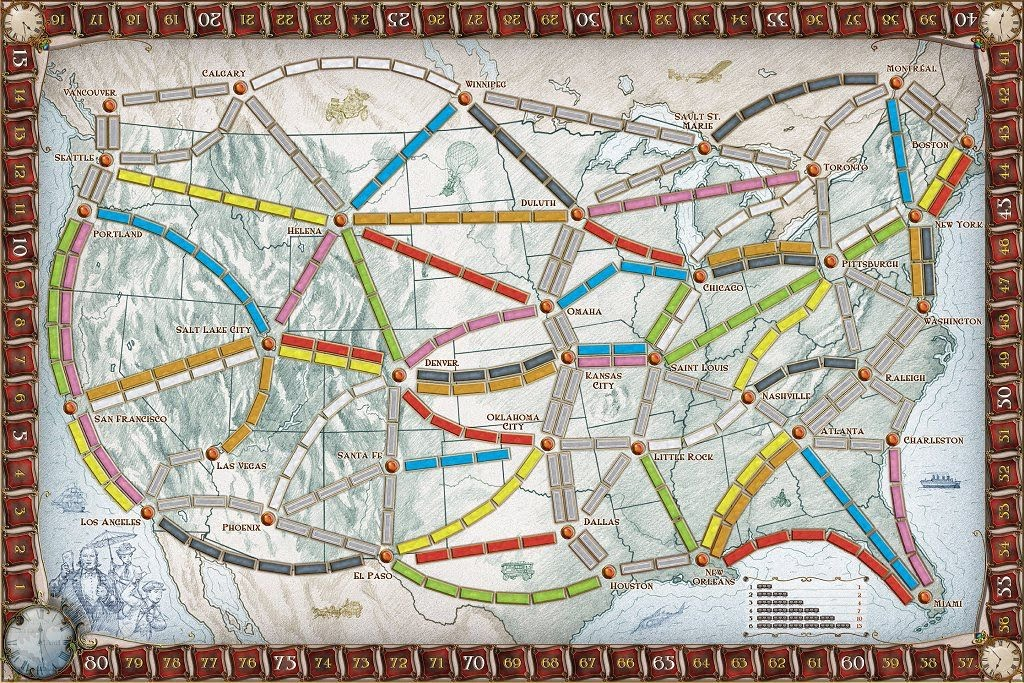
\includegraphics[scale=0.26]{figures/TTR.jpg}\ 
\end{center}
\caption{\protect\url{https://meepletown.com/wp-content/uploads/2011/03/TTR.jpg} (Retrieved on February 12, 2019)}
\end{figure}

\textbf{Note: This specification is provided as part of Assignment 2, 3 and 4 of CSCI2134 in Winter 2023 and explains what the code is supposed to do. Please see the assignment instructions for your task, e.g. writing unit tests for the code. Do not spend time writing code for the ticket to ride problem.}


\section*{Background: Ticket to Ride, the Board Game}
In a popular board game, called ``Ticket to Ride''\footnote{Published
by Days of Wonder}, the goal of the game is to build a rail network
that covers the routes each player is given.  A route is specified by
the end-point cities, and is constructed by building segments
illustrated on the game board above.  For example, to build a route
between Boston and Winnipeg, a player may choose to build the
segments: Boston to Montreal, Montreal to Toronto, Toronto to Duluth,
and Duluth to Winnipeg.  The longer the segments the more expensive they
are to build, and routes with more segments take longer to build.
Thus, it is in the player's interest to build the routes she is allocated
in the most efficient way possible.  

\section*{Problem: Minimize Network Length}
Given a game board of rail segments and a list of routes, your task
is to compute the total cost of building a network of prescribed
routes, assuming that the shortest distance for each route is chosen.

For example, given the following game board and routes:
\begin{figure}[h]
\begin{quote}
\begin{verbatim}
Boston 2 Montreal
Boston 2 New_York
Chicago 4 Toronto
Chicago 3 Pittsburgh
Montreal 3 New_York
Montreal 3 Toronto
New_York 2 Washington
New_York 2 Pittsburgh
Pittsburgh 2 Toronto
Pittsburgh 2 Washington
done
Washington Montreal
Chicago New_York
done
\end{verbatim}
\end{quote}
\caption{Sample of possible rail segments and two routes.  \label{fig:input}}
\end{figure}

The resulting cost computation would be:
\begin{figure}[h]
\begin{quote}
\begin{verbatim}
The rail network consists of:
  Chicago 3 Pittsburgh
  Montreal 3 New_York
  New_York 2 Pittsburgh
  New_York 2 Washington
The total cost is: 10
\end{verbatim}
\end{quote}
\caption{Segments and total cost of building a rail network for the specified
         routes and game board in Figure~\ref{fig:input} \label{fig:output}}
\end{figure}


Your task is to create a program that reads a game board and routes,
and computes which segments should be constructed and the total cost.

Write a program called {\tt RouteCost.java} that reads in a
game board and routes from the console ({\it
System.in}) and outputs the set of segments to be built and 
the total cost.

\subsection*{Input}
Your program should read in the input using a {\it Scanner} object,
which is instantiated with {\it System.in}.  The input will comprise
two sections with one or more lines in each section.   The first
section contains the game board and comprises zero or more lines
of the form
\begin{quote}
$C_1$ $L$ $C_2$
\end{quote}
where $C_1$ and $C_2$ are the end-points of a segment on the game board and
$L$ is the length of the segment.  E.g., ``{\tt Toronto 3 Montreal}''.  The 
section is terminated by a single word ``{\tt done}''.

The second section contains the routes and comprises zero or more
lines of the form
\begin{quote}
$C_1$ $C_1$
\end{quote}
where $C_1$ and $C_2$ are the end-points of a route, comprising one
or more segments.   E.g., ``{\tt Montreal Washington}''.  The section
is terminated by a single word ``{\tt done}''.

Hint:  All you need to use are the {\tt next()} and {\tt nextInt()}
methods of the {\it Scanner} object.


\subsection*{Semantics}
The game board is connected and all the city names are single words,
e.g., ``\verb%Las_Vegas%''.  You may assume that all game boards
and all routes will be valid.  All routes will have distinct
end-points (no cycles or 0-length routes).

The segments are bidirectional, i.e., can be used in either direction,
and the game board represents a weighted undirected graph.  Routes
may intersect and may share segments.  Segments need only be counted
once though.

The cost of a route is the sum of the lengths of the segments
in the route.  A rail network is considered minimal if each route
has minimum cost.  

\subsection*{Output}
Your program should output to {\it System.out}.  Each line should be
terminated by a new line character.  The output should begin with the 
line:
\begin{quote}
\tt The rail network consists of:
\end{quote}
followed by the list of segments used in the rail network.  Each
segment should be indented two (2) spaces, and the segments should
be in sorted order, where the $(C_1,L,C_2)$ precedes $(C'_1,L',C'_2)$
if $C_1$ lexically precedes $C'_1$, or if $C_1$ equals $C'_1$, then
$C_2$ must lexically precede $C'_2$.  The format of the segments is the
same format as the input.  

The list of segments should be followed by the line
\begin{quote}
\tt The total cost is: $T$
\end{quote}
where $T$ is the sum of lengths of the segments.
See Figure~\ref{fig:output} for an example.  


\subsection*{Example}
% Below are a sequence of examples and the corresponding output.

\begin{tabular}{l|l}
{\bf Sample Input } & {\bf Sample Output} \\
\hline
\begin{minipage}[t]{0.5\linewidth}
\vspace*{0.5ex}
\begin{verbatim}
Charleston 2 Raleigh
Chicago 3 Pittsburgh
Chicago 2 Saint_Louis
Chicago 4 Omaha
Chicago 3 Duluth
Dallas 2 Little_Rock
Dallas 2 Oklahoma_City
Denver 4 Omaha
Denver 4 Kansas_City
Denver 4 Oklahoma_City
Denver 2 Santa_Fe
Denver 3 Salt_Lake_City
Duluth 2 Omaha
Duluth 6 Helena
Helena 4 Winnipeg
Helena 5 Omaha
Helena 4 Denver
Helena 3 Salt_Lake_City
Kansas_City 2 Saint_Louis
Kansas_City 2 Oklahoma_City
Kansas_City 1 Omaha
Las_Vegas 3 Salt_Lake_City
Little_Rock 3 Nashville
Little_Rock 2 Oklahoma_City
Little_Rock 2 Saint_Louis
Nashville 3 Raleigh
Nashville 2 Saint_Louis
Nashville 4 Pittsburgh
New_York 2 Washington
New_York 2 Pittsburgh
Oklahoma_City 3 Santa_Fe
Pittsburgh 2 Washington
Pittsburgh 2 Raleigh
Pittsburgh 5 Saint_Louis
Raleigh 2 Washington
Saint_Louis 2 Chicago
done
Denver Washington
Chicago Oklahoma_City
done
\end{verbatim}
\vspace*{0.5ex}
\end{minipage} &
\begin{minipage}[t]{0.4\linewidth}
\vspace*{0.5ex}
\begin{verbatim}
The rail network consists of:
  Chicago 2 Saint_Louis
  Denver 4 Kansas_City
  Kansas_City 2 Saint_Louis
  Little_Rock 2 Oklahoma_City
  Little_Rock 2 Saint_Louis
  Nashville 3 Raleigh
  Nashville 2 Saint_Louis
  Raleigh 2 Washington
The total cost is: 19
\end{verbatim}
\end{minipage} \\
\end{tabular}

\section*{Hints and Suggestions}
\begin{itemize}\NoItemSpace
\item Use a 2-phase algorithm:  Create a weighted graph representing
      the game board.  Then, use Dijkstra's shortest weighted path algorithm
      to find the shortest routes.
\item The sample solution is under 200 lines of code.
% \item Your code {\bf must} compile.  If it does not compile, you will
%       receive a $0$ on the assignment.
\item Your code must be well commented and indented.  Please see the
      Assignments section for this course on Brightspace for Code 
      Style Guidelines.
\item You may assume that all input will be correct.  
\item Be sure to test your programs using the provided tests or {\it Mimir}.
\end{itemize}


\end{document}
